The Hazard Modeller's Toolkit (or ``hmtk'') is a Python library of functions written by scientists at the GEM Model Facility, which is intended to provide 
scientists and engineers with the tools to help create the seismogenic 
input models that go into the OpenQuake hazard engine. The process of 
developing building the hazard model is a complex and often challenging 
one, and whilst many aspect of the practice are relatively common, the 
choice of certain methods or tools for undertaking each step can be a 
matter of judgement. The intention of this software is to provide 
scientists and engineers with the means to apply many of the most 
commonly used algorithms for preparing seismogenic source models 
using seismicitiy and geological data. It is still in an early 
stage of development and the current versions contain only a preliminary
set of tools for undertaking the necessary workflows. In forthcoming 
versions will hope to make available more tools for the current processes
indicated here, and to integrate new functionalities for i) merging and
homogenisation of earthquake catalogues, ii) calculation of activity 
rates from geological and geodetic data, iii) testing and interpretation
of Ground Motion Prediction Equations, and iv) integration of 
seismological and geological data and treatment of uncertainty 
in the construction of seismogenic source zones.

\section{Getting Started and Running the Software}
The Modeller's Toolkit and associated software are designed for execution 
from the command line. As with OpenQuake, the preferred environment is 
Ubuntu Linux (11.04 or later). A careful effort has been made to keep 
the number of additional dependencies to a minimum. No packaged version of the software has been released at the time of writing, so the user must install the dependencies manually. More information regarding the current dependencies of the toolkit can be found at \hfill \\
\href{http://github.com/GEMScienceTools/hmtk}{http://github.com/GEMScienceTools/hmtk}. 

The current dependencies are:
\begin{itemize}
\item Numpy and Scipy (included in the standard OpenQuake installation)
\item Shapely (included in the standard OpenQuake installation)
\item Openquake nrmllib (included in the standard OpenQuake installation) 
    \hfill \\ (\href{http:/github.com/gem/oq-nrmllib}{http:/github.com/gem/oq-nrmllib}) 
\item Openquake hazardlib (included in the standard OpenQuake installation) 
    \hfill \\ (\href{http:/github.com/gem/oq-hazardlib}{http:/github.com/gem/oq-hazardlib})
\item Matplotlib (\href{http://matplotlib.org/}{http://matplotlib.org/})
\item PyYaml
\end{itemize}

The Matplotlib and Pyyaml dependencies are installed in the library for the demos, but can be installed easy from the command line by:
\begin{Verbatim}[frame=single, commandchars=\\\{\}, fontsize=\scriptsize]

~\$ sudo pip install matplotlib
~\$ sudo pip instal pyyaml

\end{Verbatim}

\textbf{For the purposes of the current exercises all of the Modeller's Toolkit dependencies have been installed in both the OpenQuake .ova files and on the OATS server - so no installation is necessary! For instructions on how to install OpenQuake and the Modeller's Toolkit, please refer to the appendix of this document}

As mentioned, the Modeller's Toolkit itself is a Python library. This means that its functions can be utlised in many different python applications. It is not, at present, a stand-alone software, and requires some investment of time from the user to understand the functionalities and learn how to link the various tools together into a workflow that will be suitable for the modelling problem at hand. For the current exercise of preparing seismic hazard inputs for sources in Nepal, a "wrapper" script has been prepared that links together a common workflow: 

\begin{enumerate}

\item Starting with a single magnitude-homogenised earthquake catalogue apply a declustering algorithm to identify and remove non-Poissonian events

\item For the declustered catalogue, use a statistical methodology to determine the time variation in completeness. Currently only the methodology of \cite{Stepp1971} is implemented.

\item With the completeness periods of the catalogue known calculate a \cite{GutenbergRichter1944} recurrence model (a- and b-value with uncertainties) for either the catalogue as a whole, or for earthquakes selected within certain area zones.

\item Implementation of a statistical estimator of maximum magnitude from the earthquake catalogue  

\end{enumerate}

In addition to this wrapper script, I also include snippets of code to show how the individual functions can be invoked and executed. To execute the snippets you will need to use the "Interactive Python" (IPython) environment. This will need to be installed from the python package repository:

\begin{Verbatim}[frame=single, commandchars=\\\{\}, fontsize=\scriptsize]

~\$ sudo pip install ipython

\end{Verbatim}

An "interactive" session can then be opened by typing \verb=ipython= at the command prompt. If matplotlib is installed and you want to make use of one or two of the plotting functionalities then you should open ipython with \verb=ipython --pylab=. To exit an ipython session at any time simply type \verb=exit=.

The Modeller's Toolkit itself requires no specific installation. In a Unix/Linux environment you can simply download the code as a zipped package from the website shown previously, then unzip and move into the code directory.
Alternatively you can download the code directly into  any current repository with the command

\begin{Verbatim}[frame=single, commandchars=\\\{\}, fontsize=\scriptsize]

~\$ git clone https://github.com/GEMScienceTools/hmtk.git

\end{Verbatim}


The execution of the Modeller's Toolkit is done from within the main directory in which the code is contained. The selection of the algorithm and the general configuration of the software is done via a configuration file (in this example \verb=Nepal_hmtk_demo_config.yml=. This is a YAML (Yet Another Markup Language) file, which can be opened and edited with any common text editor (e.g. vi, emacs, gedit).

To run the Nepal "wrapper" code for the Modeller's Toolkit simply move into the directory in which the \verb=main.py= file is found. Once the configuration file is correctly set up, execute via the following command:
\begin{Verbatim}[frame=single, commandchars=\\\{\}, fontsize=\scriptsize]
~\$ python hmtk_Nepal_Demo.py --input=Nepal_hmtk_demo_config.yml
\end{Verbatim}

%The \verb=-d= indicates that the program can be run in ''debug'' mode. This will create a log (written automatically to the file \verb=debug.log=) of the processes that are executed inside the toolkit in addition to certain parameters that may be calculated at intermediate steps of the process, but are not written to the output. The \verb=-d= can be omitted if preferred, in which case the program will return only a minimal indication of the progress to the command prompt.

\subsection{Nepal Demonstration: The Configuration File}

The following demonstration is designed to illustrate how the toolkit could be used to help build a hazard model using current data (and seismogenic sources) for Nepal and the surrounding regions. The data and the study area are shown in Figure \ref{fig:KathGSHAPLabel}

\begin{figure}[htbp]
	\centering
		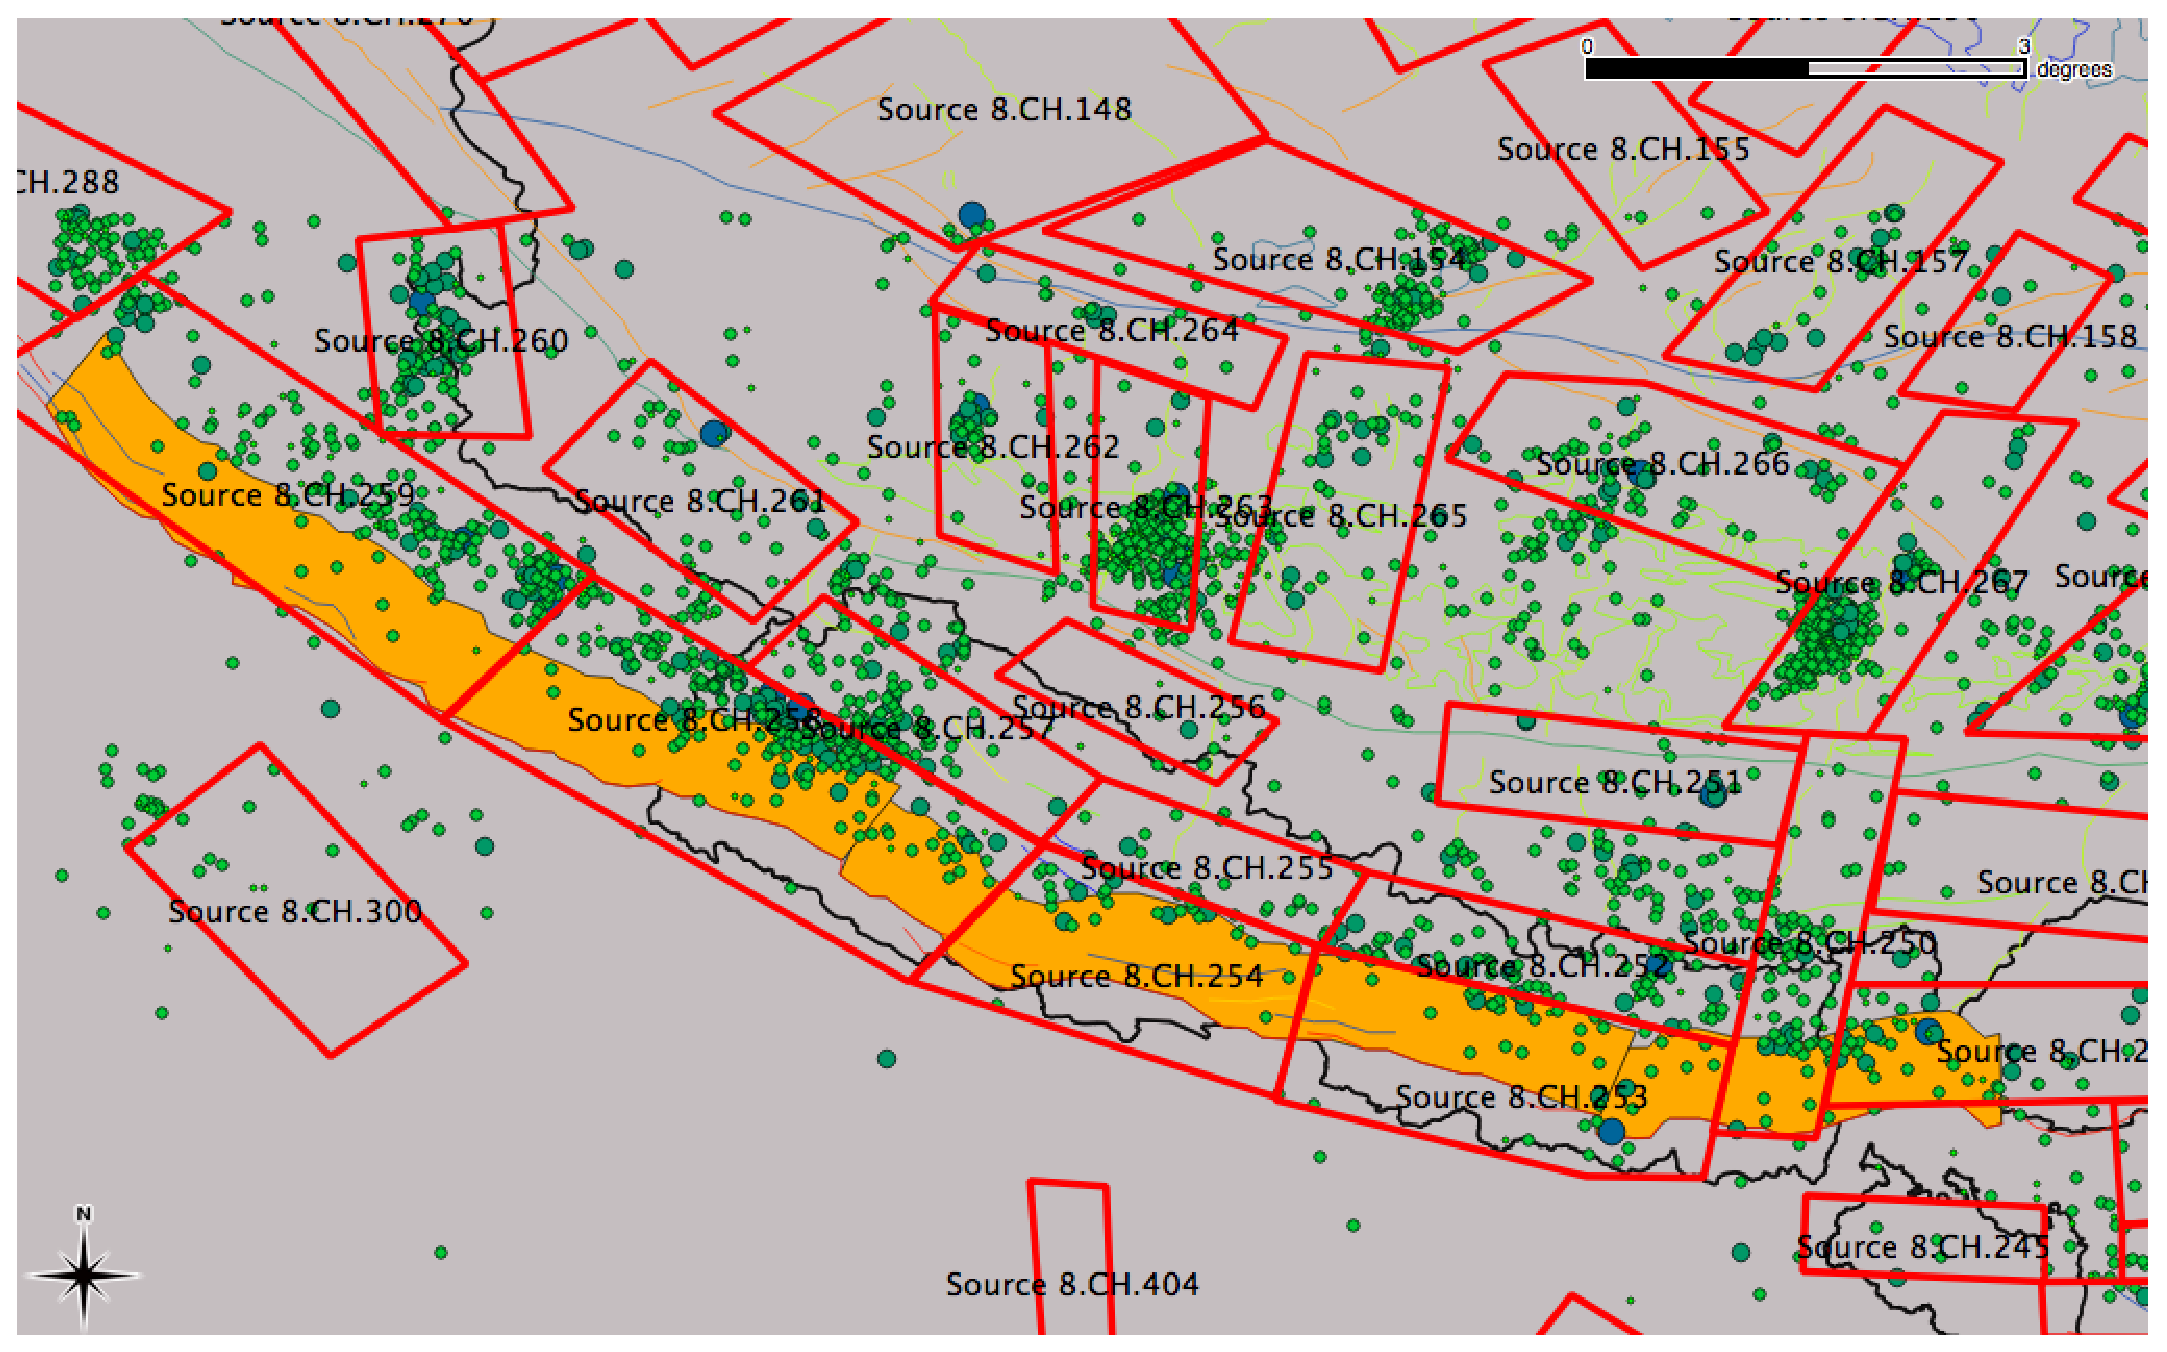
\includegraphics[width=15cm, keepaspectratio=true]{./figures/Kathmandu_plus_GSHAP_sources_labelled.eps}
	\caption{Seismotectonic Information for Nepal and the Surroundings. Earthquakes catalogue taken from the International Seismological Centre, Area Sources (red) from GSHAP and active fault sources (including surface projections for the Main Boundary Thrust (orange)) from \cite{TaylorYin2009}}
	\label{fig:KathGSHAPLabel}
\end{figure}






